\documentclass[9pt,aspectratio=169,xcolor=table]{beamer}

%~~~~~~~~~~~~~~~~~~~~~~~~~~~~~~~~~~~~~~~~~~~~~~~~~~~~~~~~~~~~~~~~~~~~~~~~~~~~~~
% Use roboto Font (recommended)
\usepackage[sfdefault]{roboto}
\usepackage[utf8]{inputenc}
\usepackage[T1]{fontenc}
%~~~~~~~~~~~~~~~~~~~~~~~~~~~~~~~~~~~~~~~~~~~~~~~~~~~~~~~~~~~~~~~~~~~~~~~~~~~~~~

%~~~~~~~~~~~~~~~~~~~~~~~~~~~~~~~~~~~~~~~~~~~~~~~~~~~~~~~~~~~~~~~~~~~~~~~~~~~~~~
% Define where theme files are located. ('/styles')
\usepackage{styles/fluxmacros}
\usefolder{styles}
% Use Flux theme v0.1 beta
% Available style: asphalt, blue, red, green, gray
% "red" is the closest built-in style to maroon; its exact colours are
% overridden with a true maroon palette just below, after the theme loads.
\usetheme[style=red]{flux}
%~~~~~~~~~~~~~~~~~~~~~~~~~~~~~~~~~~~~~~~~~~~~~~~~~~~~~~~~~~~~~~~~~~~~~~~~~~~~~~

%~~~~~~~~~~~~~~~~~~~~~~~~~~~~~~~~~~~~~~~~~~~~~~~~~~~~~~~~~~~~~~~~~~~~~~~~~~~~~~
% SKEE1033 maroon palette override.
% The flux theme's colortheme defines primaryLight/primary/secondary/tertiary
% as plain \definecolor calls (not \providecolor), so simply redefining them
% here, AFTER \usetheme, wins -- xcolor allows redefinition and every
% \setbeamercolor in beamercolorthemeflux.sty was already evaluated against
% these names, so the redefinition propagates everywhere automatically.
\definecolor{primaryLight}{HTML}{9B2242} % lighter maroon -- headers, accents
\definecolor{primary}{HTML}{7B1E3A}      % core maroon -- titles, block headers
\definecolor{secondary}{HTML}{3A5A6B}    % muted teal -- complementary accent
\definecolor{tertiary}{HTML}{8C6A3F}     % warm bronze -- example/third accent
%~~~~~~~~~~~~~~~~~~~~~~~~~~~~~~~~~~~~~~~~~~~~~~~~~~~~~~~~~~~~~~~~~~~~~~~~~~~~~~

%~~~~~~~~~~~~~~~~~~~~~~~~~~~~~~~~~~~~~~~~~~~~~~~~~~~~~~~~~~~~~~~~~~~~~~~~~~~~~~
% Extra packages
\usepackage{booktabs}
\usepackage{colortbl}
\usepackage{ragged2e}
\usepackage{amssymb}
\usepackage{multirow}
\usepackage{tikz}
\usetikzlibrary{arrows.meta, positioning, fit, backgrounds, calc, shapes.geometric}
\usepackage{circuitikz}
\setbeamertemplate{itemize items}[square]
\usepackage[scaled=.92]{beramono}
\usepackage{listings}
\usepackage{array}
% Table striping: odd rows white, even rows very light gray.
\definecolor{stripe}{gray}{0.94}
\newcommand{\striped}{\rowcolors{1}{white}{stripe}}
%~~~~~~~~~~~~~~~~~~~~~~~~~~~~~~~~~~~~~~~~~~~~~~~~~~~~~~~~~~~~~~~~~~~~~~~~~~~~~~

%~~~~~~~~~~~~~~~~~~~~~~~~~~~~~~~~~~~~~~~~~~~~~~~~~~~~~~~~~~~~~~~~~~~~~~~~~~~~~~
% Code listing style (lightweight analogue of the book's skpython style).
% This course is Python-only, so Python is set as the lstlisting default via
% \lstset below -- every \begin{lstlisting} needs no language=... of its own.
\definecolor{codebg}{HTML}{FBF2F4}
\definecolor{codegreen}{rgb}{0,0.45,0}
\definecolor{codestring}{rgb}{0.58,0.1,0.2}
\lstdefinestyle{skpython}{
    basicstyle=\ttfamily\footnotesize,
    keywordstyle=\color{primary}\bfseries,
    commentstyle=\itshape\color{codegreen},
    stringstyle=\ttfamily\color{codestring},
    backgroundcolor=\color{codebg},
    breaklines=true,
    keepspaces=true,
    showspaces=false,
    showstringspaces=false,
    frame=single,
    rulecolor=\color{primary!40},
    numbers=none,
}
\lstset{language=Python, style=skpython}

% Console-output style: distinguishes program output from source code.
\lstdefinestyle{skoutput}{
    basicstyle=\ttfamily\footnotesize,
    backgroundcolor=\color{secondary!8},
    breaklines=true,
    frame=single,
    rulecolor=\color{secondary!50},
    numbers=none,
}
\lstnewenvironment{pyout}{\lstset{style=skoutput, language={}}}{}
%~~~~~~~~~~~~~~~~~~~~~~~~~~~~~~~~~~~~~~~~~~~~~~~~~~~~~~~~~~~~~~~~~~~~~~~~~~~~~~

%~~~~~~~~~~~~~~~~~~~~~~~~~~~~~~~~~~~~~~~~~~~~~~~~~~~~~~~~~~~~~~~~~~~~~~~~~~~~~~
% TikZ block styles for the workflow and control-structure diagrams
\definecolor{cycfill}{HTML}{F3DCE4}
\definecolor{cycline}{HTML}{7B1E3A}
\definecolor{cycdofill}{HTML}{E8EEF0}
\definecolor{cycdoline}{HTML}{3A5A6B}
\tikzset{
  cycstep/.style = {font=\sffamily\small, align=center, rounded corners=2pt,
                     draw=cycline, fill=cycfill, line width=0.7pt,
                     minimum height=7mm, minimum width=20mm, inner sep=3pt},
  cycdo/.style   = {cycstep, fill=cycdofill, draw=cycdoline},
  flow/.style    = {-{Stealth[length=2mm]}, thick, draw=cycline},
}
%~~~~~~~~~~~~~~~~~~~~~~~~~~~~~~~~~~~~~~~~~~~~~~~~~~~~~~~~~~~~~~~~~~~~~~~~~~~~~~

%%%%%%%%%%%%%%%%%%%%%%%%%%%%%%%%%%%
%% SECTION SEPARATOR (ToC recap) %%
%%%%%%%%%%%%%%%%%%%%%%%%%%%%%%%%%%%
\AtBeginSection[]
{
{
    \setbeamercolor{background canvas}{bg=primaryLight!6}
    \begin{frame}[plain]
        \frametitle{Table of Contents}
        \tableofcontents[currentsection]
    \end{frame}
}
}
%%%%%%%%%%%%%%%%%%%%%%%%%%%%%%%%%%%

%~~~~~~~~~~~~~~~~~~~~~~~~~~~~~~~~~~~~~~~~~~~~~~~~~~~~~~~~~~~~~~~~~~~~~~~~~~~~~~
% Information
\title{Measurements, Files and Spreadsheets}
\subtitle{\emph{Engineering Computation with Python} --- Chapter 10}
\author{Mun\'{i}m Zabidi}
\institute{\color{primary}Faculty of Electrical Engineering, Universiti Teknologi Malaysia}
\date{\today}
\titlegraphic{assets/logoutmwhite.png}
%~~~~~~~~~~~~~~~~~~~~~~~~~~~~~~~~~~~~~~~~~~~~~~~~~~~~~~~~~~~~~~~~~~~~~~~~~~~~~~

\begin{document}

\titlepage

\begin{frame}{Table of Contents}
    \tableofcontents
\end{frame}

%===============================================================================
\section{From the Console to a File}
%===============================================================================

\begin{frame}{Two Ways Data Reaches a Python Program}
    \leavevmode
    Up to now, every number in your programs was typed directly into the
    code. Real engineering data arrives differently.

    \vspace{3mm}
    \begin{columns}[t]
        \begin{column}{.48\textwidth}
            \begin{block}{Prompt data}
                \small Entered or displayed at the console while a
                script runs. Temporary --- it disappears once the
                program closes.
            \end{block}
        \end{column}
        \begin{column}{.48\textwidth}
            \begin{block}{Import/export data}
                \small Stored in a file (\texttt{.csv}, \texttt{.xlsx},
                \texttt{.txt}, \ldots). Permanent, shareable, and
                usually larger.
            \end{block}
        \end{column}
    \end{columns}

    \vspace{4mm}
    \begin{alertblock}{This chapter's purpose}
        Close the gap between a laboratory measurement and a Python
        calculation --- both directions.
    \end{alertblock}
\end{frame}

\begin{frame}{The Workflow Is Always the Same}
    \leavevmode
    \begin{center}
    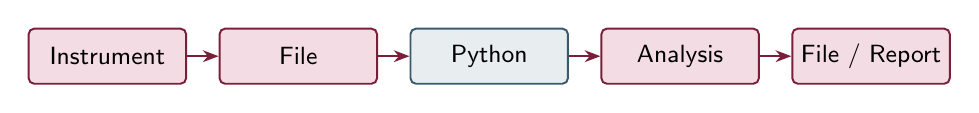
\begin{tikzpicture}[node distance=6mm and 4mm]
        \node[cycstep] (inst) {Instrument};
        \node[cycstep, right=of inst] (file1) {File};
        \node[cycdo,   right=of file1] (py)   {Python};
        \node[cycstep, right=of py]   (an)   {Analysis};
        \node[cycstep, right=of an]   (file2) {File / Report};
        \draw[flow] (inst)  -- (file1);
        \draw[flow] (file1) -- (py);
        \draw[flow] (py)    -- (an);
        \draw[flow] (an)    -- (file2);
    \end{tikzpicture}
    \end{center}

    \vspace{4mm}
    Consider the bench recording from earlier chapters. Loading it
    takes one line, and the first thing to do afterwards is always to
    \alert{look at what arrived}.
\end{frame}

\begin{frame}[fragile]{Loading and Checking a Real Recording}
    \leavevmode
\begin{lstlisting}
import pandas as pd

data = pd.read_csv('bench_rc.csv')
print(data.shape)     # (101, 4)
print(data.head(3))
\end{lstlisting}

    \vspace{2mm}
    \textbf{Engineering sanity checks, every time:}
    \begin{itemize}\small
        \item \textbf{Shape.} 101 rows at $20\,\text{ms}$ covers two
              seconds --- matches the experiment.
        \item \textbf{Units.} Column names carry them: volts,
              milliamps, \textcelsius.
        \item \textbf{Magnitude.} First current $2.55\,\text{mA}$
              matches $12\,\text{V}/4.7\,\text{k}\Omega$.
        \item \textbf{Completeness.} \texttt{data.isna().sum()} finds
              the logger dropout.
    \end{itemize}
\end{frame}

\begin{frame}[fragile]{Requesting Input from the User}
    \leavevmode
    \texttt{input()} always returns a \alert{string} --- numeric
    responses must be converted explicitly.

\begin{lstlisting}
text   = input("Enter a text: ")
number = float(input("Enter a number: "))
\end{lstlisting}

    \vspace{2mm}
    \begin{columns}[t]
        \begin{column}{.5\textwidth}
\begin{lstlisting}
height = float(input('Enter height: '))
width  = float(input('Enter width: '))
area = 0.5 * width * height
print(f'Area = {area}')
\end{lstlisting}
        \end{column}
        \begin{column}{.45\textwidth}
            \small Console session:
\begin{pyout}
Enter height: 10
Enter width: 20
Area = 100.0
\end{pyout}
        \end{column}
    \end{columns}
\end{frame}

\begin{frame}[fragile]{Three Ways to Display a Value}
    \leavevmode
    \begin{columns}[t]
        \begin{column}{.33\textwidth}
            \begin{block}{Direct display}
                \scriptsize
\begin{lstlisting}
x = 10
x
\end{lstlisting}
                \tiny\texttt{10}
            \end{block}
        \end{column}
        \begin{column}{.33\textwidth}
            \begin{block}{print()}
                \scriptsize
\begin{lstlisting}
x = 10
print(x)
\end{lstlisting}
                \tiny\texttt{10}
            \end{block}
        \end{column}
        \begin{column}{.33\textwidth}
            \begin{block}{print() + f-string}
                \scriptsize
\begin{lstlisting}
x = 10
print(f'x is {x}')
\end{lstlisting}
                \tiny\texttt{x is 10}
            \end{block}
        \end{column}
    \end{columns}

    \vspace{4mm}
    \begin{alertblock}{The difference}
        Direct display and \texttt{print()} show only the value. An
        f-string lets the output include \alert{explanatory text}
        along with it --- the next section develops this fully.
    \end{alertblock}
\end{frame}

%===============================================================================
\section{Formatted Output with f-Strings}
%===============================================================================

\begin{frame}[fragile]{Controlling How a Value Looks}
    \leavevmode
    An f-string offers far more control than a basic \texttt{print()}:
    width, decimal places, and notation --- all inside the braces.

\begin{lstlisting}
formatted_string = f"text {variable1:.2f} more text {variable2:d}"
\end{lstlisting}

    \vspace{2mm}
    \begin{itemize}
        \item Curly braces \texttt{\{\}} are placeholders for variables.
        \item A \alert{format specifier} after the colon controls
              width and precision (e.g.\ \texttt{.2f} = 2 decimal
              places).
        \item Formatting affects only \alert{display} --- never the
              stored value.
    \end{itemize}
\end{frame}

\begin{frame}{Common Format Specifiers}
    \leavevmode
    \small
    \striped
    \begin{tabular}{@{}p{0.2\linewidth}cp{0.22\linewidth}p{0.35\linewidth}@{}}
        \toprule
        \textbf{Value Type} & \textbf{Code} & \textbf{Example} & \textbf{Meaning} \\
        \midrule
        Integer & \texttt{d} & \texttt{\{v:d\}} & Signed decimal integer \\
        Float & \texttt{f} & \texttt{\{v:7.2f\}} & Width 7, 2 decimal places \\
        String & \texttt{s} & \texttt{\{v:s\}} or \texttt{\{v\}} & Plain string output \\
        Scientific & \texttt{e}/\texttt{E} & \texttt{\{v:e\}} & Exponential notation \\
        \bottomrule
    \end{tabular}
\end{frame}

\begin{frame}[fragile]{A Single Value, Several Ways}
    \leavevmode
\begin{lstlisting}
cows = 5
print(f'There are {cows:7.2f} cows in the pasture')
\end{lstlisting}

\begin{pyout}
There are    5.00 cows in the pasture
\end{pyout}

    \vspace{2mm}
    \begin{block}{Reading \texttt{\{cows:7.2f\}}}
        \texttt{7} sets a minimum field width of 7 characters
        (digits, point, and padding). \texttt{.2f} sets 2 decimal
        places.
    \end{block}
\end{frame}

\begin{frame}[fragile]{Formatting Several Values at Once}
    \leavevmode
    Consistent column widths are what make a printed table readable:

\begin{lstlisting}
L = [[20, 3.3], [20000, 3300]]
print(f'{L[0][0]:2.2f}m is equivalent to {L[1][0]:5d}mm')
print(f'{L[0][1]:2.2f}m is equivalent to {L[1][1]:5d}mm')
\end{lstlisting}

\begin{pyout}
20.00m is equivalent to 20000mm
3.30m is equivalent to  3300mm
\end{pyout}

    \vspace{1mm}
    {\small A 2D list is indexed \texttt{L[row][column]} --- double
    brackets, not \texttt{L[row, column]}.}
\end{frame}

%===============================================================================
\section{Files: Text, Binary, and Beyond}
%===============================================================================

\begin{frame}{Import, Export, Text, Binary}
    \leavevmode
    \begin{columns}[t]
        \begin{column}{.5\textwidth}
            \begin{block}{Direction}
                \small
                \begin{itemize}
                    \item \textbf{Import} --- disk $\to$ Python
                    \item \textbf{Export} --- Python $\to$ disk
                \end{itemize}
            \end{block}
        \end{column}
        \begin{column}{.5\textwidth}
            \begin{block}{Representation}
                \small
                \begin{itemize}
                    \item \textbf{Text} --- readable (CSV, TXT, JSON)
                    \item \textbf{Binary} --- not readable in a text
                          editor (images, audio, serialized objects)
                \end{itemize}
            \end{block}
        \end{column}
    \end{columns}

    \vspace{4mm}
    \begin{alertblock}{The pattern, regardless of format}
        \texttt{open()} creates a file object; \texttt{read()} and
        \texttt{write()} move data through it. Everything that
        follows is a variation on this one idea.
    \end{alertblock}
\end{frame}

\begin{frame}[fragile]{Reading and Writing Plain Text}
    \leavevmode
\begin{lstlisting}
# Writing to a text file
with open('example.txt', 'w') as file:
    file.write('Hello, World!')

# Reading from a text file
with open('example.txt', 'r') as file:
    content = file.read()
    print(content)  # Output: Hello, World!
\end{lstlisting}

    \vspace{2mm}
    \begin{block}{The \texttt{with} statement}
        Opens the file, hands it to \texttt{file}, and \alert{closes
        it automatically} when the block ends --- even if an error
        occurs inside.
    \end{block}
\end{frame}

\begin{frame}[fragile]{Binary Data: Same Pattern, Different Mode}
    \leavevmode
    Adding \texttt{b} to the mode writes raw bytes --- for data not
    meant to be read by eye, like instrument recordings.

    \begin{columns}[t]
        \begin{column}{.48\textwidth}
            \scriptsize \textbf{Serializing a Python object:}
\begin{lstlisting}
import pickle
data = {'key': 'value'}
with open('data.pkl', 'wb') as f:
    pickle.dump(data, f)

with open('data.pkl', 'rb') as f:
    loaded = pickle.load(f)
\end{lstlisting}
        \end{column}
        \begin{column}{.48\textwidth}
            \scriptsize \textbf{Saving a NumPy array:}
\begin{lstlisting}
import numpy as np
arr = np.array([1, 2, 3])
np.save('array.npy', arr)

loaded = np.load('array.npy')
\end{lstlisting}
        \end{column}
    \end{columns}

    \vspace{2mm}
    {\small \texttt{pickle} serializes any Python object;
    \texttt{numpy.save}/\texttt{load} is the NumPy-specific
    equivalent.}
\end{frame}

\begin{frame}{Choosing a Format: When to Use What}
    \leavevmode
    \small
    \begin{itemize}
        \item \textbf{Text file} (\texttt{open}, \texttt{read},
              \texttt{write}) --- small, human-readable notes or logs.
        \item \textbf{pickle} --- saving an arbitrary Python object
              (a dictionary, a trained model) exactly as it was.
        \item \textbf{NumPy \texttt{.npy}} --- saving a large array
              efficiently, without converting to text.
        \item \textbf{CSV / spreadsheet} --- tabular measurement data
              meant to be shared, inspected, or opened in Excel.
    \end{itemize}

    \vspace{3mm}
    \begin{block}{This chapter's focus}
        Spreadsheets and CSV are the formats engineers meet daily ---
        the rest of this chapter covers them in depth.
    \end{block}
\end{frame}

%===============================================================================
\section{Spreadsheets and CSV}
%===============================================================================

\begin{frame}[fragile]{Reading and Writing a Spreadsheet: Syntax}
    \leavevmode
\begin{lstlisting}
# Reading data
data = pd.read_excel(filename, sheet_name='Sheet1',
                      usecols='B:Z', header=None)

# Selecting rows/columns
selected_data = data.iloc[1, 1:]

# Writing data back
output_data.to_excel(filename, sheet_name='Sheet1',
                      startcol=1, startrow=2,
                      index=False, header=False)
\end{lstlisting}

    \vspace{1mm}
    {\small \texttt{startcol}/\texttt{startrow} target where writing
    begins; \texttt{index=False} skips saving the DataFrame's row
    index into the sheet.}
\end{frame}

\begin{frame}[fragile]{Worked Example: Celsius to Fahrenheit}
    \leavevmode
    A room temperature log sits in \texttt{tempData.xlsx}. Convert
    every reading to Fahrenheit and append it to the same file.

\begin{lstlisting}
temp_c = pd.read_excel(file_path, sheet_name='Sheet1',
                        header=None).iloc[1, 1:]
temp_f = temp_c * 9/5 + 32

with pd.ExcelWriter(file_path, engine='openpyxl', mode='a',
                     if_sheet_exists='overlay') as writer:
    output_data = pd.DataFrame([temp_f])
    output_data.to_excel(writer, sheet_name='Sheet1',
                          startcol=1, startrow=2,
                          index=False, header=False)
\end{lstlisting}

    {\small \texttt{mode='a'} with \texttt{if\_sheet\_exists=
    'overlay'} adds data \alert{without erasing} what is already
    there.}
\end{frame}

\begin{frame}{Excel vs.\ CSV: Same Idea, Fewer Moving Parts}
    \leavevmode
    \small
    \striped
    \begin{tabular}{@{}p{0.25\linewidth}p{0.32\linewidth}p{0.32\linewidth}@{}}
        \toprule
        \textbf{Feature} & \textbf{Excel} & \textbf{CSV} \\
        \midrule
        Library & \texttt{openpyxl} required & Only \texttt{pandas} \\
        Reading & \texttt{pd.read\_excel(...)} & \texttt{pd.read\_csv(...)} \\
        Writing & \texttt{pd.ExcelWriter(...)} & \texttt{.to\_csv(...)} \\
        Sheets & \texttt{sheet\_name} & None \\
        Write mode & Overlay existing cells & Append a new row \\
        Cell targeting & \texttt{startrow}, \texttt{startcol} & Not supported \\
        \bottomrule
    \end{tabular}

    \vspace{3mm}
    \begin{alertblock}{CSV is the default for measured data}
        Simpler, universally readable, and exactly what a data
        logger or lab instrument usually exports.
    \end{alertblock}
\end{frame}

\begin{frame}[fragile]{The Same Conversion, with CSV}
    \leavevmode
\begin{lstlisting}
data = pd.read_csv(file_path, header=None)
temp_c = data.iloc[1, 1:]
temp_f = temp_c * 9/5 + 32

# CSV has no cells to target -- just append a new row
output_data = pd.DataFrame([temp_f])
output_data.to_csv(file_path, mode='a',
                    index=False, header=False)
\end{lstlisting}

    \vspace{2mm}
    {\small No sheet name, no \texttt{startrow}/\texttt{startcol} ---
    CSV has no concept of cell targeting, so the converted row is
    simply appended at the end.}
\end{frame}

%===============================================================================
\section{Case Study: Mesh Circuits}
%===============================================================================

\begin{frame}{The Problem: Ten Circuits, One Spreadsheet}
    \leavevmode
    \small
    Revisit the mesh-circuit analysis from Chapter~9, now driven
    entirely by spreadsheet data: solve $I_1$ and $I_2$ for
    \alert{ten} resistor/voltage configurations stored in
    \texttt{circuit\_analysis.xlsx}.

    \vspace{2mm}
    \begin{center}
    \begin{circuitikz}[scale=0.85, transform shape]
        \draw (0,0) to[battery2, l_=$V_1$] (0,3);
        \draw (0,3) to[R, l=$R_1$, i>^=$I_1$] (3.2,3);
        \draw (3.2,3) to[R, l=$R_3$, i>^=$I_3$] (3.2,0);
        \draw (3.2,3) to[R, l=$R_2$, i<^=$I_2$] (6.4,3);
        \draw (6.4,3) to[battery2, l_=$V_2$, invert] (6.4,0);
        \draw (0,0) -- (6.4,0);
    \end{circuitikz}
    \end{center}

    {\small The script sends \texttt{R} (resistances) and \texttt{V}
    (voltages) from the spreadsheet into a helper module,
    \texttt{mesh\_solver.py}, for each of the ten rows.}
\end{frame}

\begin{frame}{The Spreadsheet Layout}
    \leavevmode
    \small
    Columns B--D hold $R_1,R_2,R_3$; columns E--F hold $V_1,V_2$;
    columns G--H are reserved for the \alert{computed} $I_1, I_2$.

    \vspace{2mm}
    \striped
    \begin{tabular}{@{}lccccc@{}}
        \toprule
         & $R_1$ & $R_2$ & $R_3$ & $V_1$ & $V_2$ \\
        \midrule
        Set 1 & 11 & 2 & 3 & 10 & $-40$ \\
        Set 2 & 5 & 20 & 10 & 10 & $-20$ \\
        Set 3 & 16 & 16 & 16 & 20 & 20 \\
        \ldots & \ldots & \ldots & \ldots & \ldots & \ldots \\
        Set 10 & 100 & 25 & 100 & $-20$ & 10 \\
        \bottomrule
    \end{tabular}

    \vspace{3mm}
    {\small Ten rows in, ten pairs of currents out --- by hand, this
    would mean solving the same $2\times2$ system ten times.}
\end{frame}

\begin{frame}[fragile]{Step 1: Separating Resistances from Indicators}
    \leavevmode
    The \texttt{R} array packs resistor values \alert{and} which loop
    each belongs to into one array:
    \[
    R =
    \begin{bmatrix}
    R_1 & R_2 & R_3 \\
    1 & 0 & 1 \\
    0 & 1 & 1
    \end{bmatrix}
    \]

\begin{lstlisting}
def separate_ir(R):
    r = R[0, :]                   # resistor values
    i = R[1:, :].astype(bool)     # which loop each belongs to
    total_loops = R.shape[0] - 1
    return i, r, total_loops
\end{lstlisting}
\end{frame}

\begin{frame}[fragile]{Step 2: Assembling and Solving \texorpdfstring{$Ax=b$}{Ax=b}}
    \leavevmode
\begin{lstlisting}
def mesh_solver(V, R):
    i, r, M = separate_ir(R)
    Rmat = np.zeros((M, M))
    for m in range(M):
        for n in range(M):
            ind_i = np.logical_and(i[m, :], i[n, :])
            if n != m:
                Rmat[m, n] = -np.sum(r[ind_i])
            else:
                Rmat[m, n] = np.sum(r[ind_i])
    I = np.linalg.solve(Rmat, V)
    return I
\end{lstlisting}

    {\small The same operation as Chapter~9's $\mathbf{Ax=b}$ ---
    now driven entirely by data read from a file.}
\end{frame}

\begin{frame}[fragile]{Step 3: Driving It from the Spreadsheet}
    \leavevmode
\begin{lstlisting}
df = pd.read_excel(file_path, sheet_name='Sheet1')
data = df.to_numpy()
I1_list, I2_list = [], []

for row in data:
    R1, R2, R3 = row[1:4]
    V1, V2 = row[4:6]
    R = np.array([[R1, R2, R3], [1, 0, 1], [0, 1, 1]])
    V = np.array([V1, V2])
    I = mesh_solver(V, R)
    I1_list.append(I[0]); I2_list.append(I[1])
\end{lstlisting}

    {\small One loop, ten configurations solved --- the pattern
    scales to a hundred rows exactly as easily.}
\end{frame}

\begin{frame}[fragile]{Step 4: Writing the Results Back}
    \leavevmode
\begin{lstlisting}
I_values_df = pd.DataFrame({'I1': I1_list, 'I2': I2_list})

with pd.ExcelWriter(file_path, mode='a',
                     if_sheet_exists='overlay') as writer:
    I_values_df.to_excel(writer, startcol=6, startrow=1,
                          index=False, header=False)
\end{lstlisting}

    \vspace{3mm}
    \begin{alertblock}{The full cycle, completed}
        Data moved from spreadsheet $\to$ Python $\to$ spreadsheet,
        with the original columns untouched and $I_1$, $I_2$ filled
        in alongside them.
    \end{alertblock}
\end{frame}

\begin{frame}{Why This Case Study Matters}
    \leavevmode
    \small
    This case study is not really about mesh circuits --- it is a
    template for almost any engineering computation on tabular data:

    \vspace{2mm}
    \begin{enumerate}
        \item Read the spreadsheet into a DataFrame.
        \item Loop over rows, extracting the inputs each row needs.
        \item Call a tested function (\texttt{mesh\_solver}) that
              does the actual engineering calculation.
        \item Collect the results and write them back.
    \end{enumerate}

    \vspace{3mm}
    \begin{block}{The same shape reappears}
        Swap \texttt{mesh\_solver} for a stress calculation, a
        calibration curve, or a filter design, and the surrounding
        read $\to$ loop $\to$ write structure barely changes.
    \end{block}
\end{frame}

\begin{frame}{Where This Is Going}
    \leavevmode
    \small
    This chapter closed the gap between a real measurement and a
    Python calculation --- both directions, prompt and file alike.

    \vspace{3mm}
    \begin{itemize}
        \item \texttt{input()} always returns a string; convert
              explicitly before computing with it.
        \item f-strings control \alert{display}, never the stored
              value.
        \item CSV is the default interchange format for measured
              data; Excel adds sheets and cell targeting.
        \item The mesh-circuit case study is the template: read,
              loop, compute, write back.
    \end{itemize}

    \vspace{4mm}
    \begin{center}
        \large\color{primary}\textbf{Next: Errors, Missing Data and Outliers}
    \end{center}
\end{frame}

\end{document}
